%-----------------------------------------------
%  Engineer's & Master's Thesis Template
%  Copyleft by Artur M. Brodzki & Piotr Woźniak
%  Warsaw University of Technology, 2019-2022
%-----------------------------------------------

\documentclass[
    bindingoffset=5mm,  % Binding offset
    footnoteindent=3mm, % Footnote indent
    hyphenation=true    % Hyphenation turn on/off
]{src/wut-thesis}

\graphicspath{{tex/img/}}
\addbibresource{bibliografia.bib}

\usepackage{xcolor}
\usepackage{tikz}
\usetikzlibrary{decorations.pathreplacing}

% Visible marker for unwritten parts. Grep for \placeholder before submission.
\newcommand{\placeholder}[1]{\textcolor{gray}{\textit{[TODO: #1]}}}

\facultyeiti    % Wydział Elektroniki i Technik Informacyjnych
\EngineerThesis % Praca inżynierska
\langeng        % Praca w języku angielskim

\begin{document}

%------------
% Title page
%------------
\instytut{XXXXXX}
\kierunek{XXXXXX}
\specjalnosc{XXXXXX}
% Working titles -- to be agreed with the supervisor.
% With \langeng, \title is the main (English) title used on the title page
% and the English abstract; \engtitle is only used by Polish theses.
\title{
    Hybrid post-quantum key exchange in an IPsec VPN: \\
    implementation and performance evaluation
}
\engtitle{
    Hybrid post-quantum key exchange in an IPsec VPN: \\
    implementation and performance evaluation
}
\poltitle{
    Hybrydowa postkwantowa wymiana kluczy w sieci VPN IPsec: \\
    implementacja i ocena wydajności
}
\frtitle{
    Échange de clés hybride post-quantique dans un VPN IPsec : \\
    mise en œuvre et évaluation des performances
}
\author{\{Imię i Nazwisko\}}
\album{XXXXXX}
\promotor{XXXXXX}
\date{\the\year}
\maketitle

%-----------------------------------------
% Abstracts (EN, PL, FR) -- write these last
%-----------------------------------------
\cleardoublepage
\abstract \placeholder{English abstract.}
\keywords post-quantum cryptography, IPsec, IKEv2, ML-KEM, hybrid key exchange, VPN

\clearpage
\secondabstract \placeholder{Streszczenie po polsku.}
\secondkeywords kryptografia postkwantowa, IPsec, IKEv2, ML-KEM, hybrydowa wymiana kluczy, VPN

\clearpage
\thirdabstract \placeholder{Résumé en français.}
\thirdkeywords cryptographie post-quantique, IPsec, IKEv2, ML-KEM, échange de clés hybride, VPN
\finishthirdabstract

\pagestyle{plain}

%-------------------
% Table of contents
%-------------------
\cleardoublepage
\tableofcontents

%----------
% Chapters
%----------
\cleardoublepage
\pagestyle{headings}

\clearpage
\section{Introduction}
\label{sec:intro}

\subsection{Motivation}
\label{sec:intro-motivation}
\placeholder{Why VPN key exchange must migrate to post-quantum cryptography now
(harvest now, decrypt later); role of IPsec/IKEv2 in enterprise and operator networks.
Two motivating settings: IoT gateways with 10--15 year lifetimes and limited resources,
and regulated financial institutions with long data-confidentiality requirements.}

\subsection{Goal and scope of the thesis}
\label{sec:intro-goal}
\placeholder{Goal: implement hybrid post-quantum key exchange in the chosen IPsec VPN
and compare its performance with a classical configuration. Scope: key exchange only;
post-quantum authentication out of scope (see Section~\ref{sec:sota-quantum}).}

\subsection{Thesis structure}
\label{sec:intro-structure}
\placeholder{One sentence per chapter. Write last.}

\clearpage
\section{Background and state of the art}
\label{sec:sota}

This chapter introduces the protocols and standards on which the rest of the
thesis builds. It begins with the threat that large-scale quantum computers
pose to public-key cryptography and explains why the key exchange of VPN
protocols is the most urgent part to migrate. It then describes the IPsec
architecture and the Internet Key Exchange Protocol Version~2 (IKEv2), with an
emphasis on the exchanges in which key material is established or refreshed.
Finally, it reviews the IETF specifications that enable post-quantum and
hybrid key exchange in IKEv2, together with existing implementations.

%---------------------------------------------------------------------------
\subsection{The quantum threat to key exchange}
\label{sec:sota-quantum}

The security of virtually all deployed public-key cryptography rests on the
hardness of integer factorisation (RSA) or of the discrete logarithm problem in
finite fields (FFDH) and on elliptic curves (ECDH, ECDSA, EdDSA). In 1994 Shor
showed that both problems can be solved in polynomial time on a sufficiently
large quantum computer~\cite{shor1997}. A \emph{cryptographically relevant
quantum computer} (CRQC) would therefore break every classical key exchange and
signature scheme currently negotiated by IKEv2.

Symmetric primitives are affected far less. Grover's algorithm~\cite{grover1996}
offers only a quadratic speed-up for exhaustive key search, which is
compensated for by using longer keys (e.g.\ AES-256 instead of AES-128). In the
context of IPsec this means that the data plane --- ESP protected with a
symmetric AEAD cipher --- remains secure, provided that the keys feeding it were
established in a quantum-resistant way.

The two uses of public-key cryptography in a VPN handshake are not equally
urgent:
\begin{itemize}
    \item \textbf{Key exchange} is exposed to the \emph{harvest now, decrypt
    later} (HNDL) attack: an adversary records encrypted traffic today and
    decrypts it once a CRQC becomes available. Data with a long confidentiality
    lifetime is thus already at risk.
    \item \textbf{Authentication} only has to resist forgery \emph{at the
    moment} the handshake takes place. A signature broken in the future does not
    retroactively compromise past sessions.
\end{itemize}
For this reason the migration of key exchange is prioritised, and it is the
focus of this thesis.

\paragraph{Standardisation.}
In 2016 NIST launched a public process to standardise post-quantum
algorithms. In August 2024 it published the first three standards:
FIPS~203 (ML-KEM, a key-encapsulation mechanism derived from
CRYSTALS-Kyber)~\cite{fips203}, FIPS~204 (ML-DSA, a lattice-based signature
scheme)~\cite{fips204} and FIPS~205 (SLH-DSA, a stateless hash-based signature
scheme)~\cite{fips205}. In March 2025 HQC was additionally selected as a backup
KEM based on different mathematical assumptions~\cite{nistir8545}. NIST has also
proposed a transition timeline under which quantum-vulnerable algorithms at the
112-bit security level are deprecated after 2030 and disallowed after
2035~\cite{nistir8547}.

\paragraph{KEM versus Diffie--Hellman.}
ML-KEM is not a drop-in replacement for Diffie--Hellman. A KEM consists of three
algorithms: \emph{KeyGen} produces an encapsulation (public) key and
a decapsulation (private) key; \emph{Encaps} takes the encapsulation key and
outputs a shared secret together with a ciphertext; \emph{Decaps} recovers the
shared secret from the ciphertext. The roles are asymmetric --- one party
sends a public key, the other answers with a ciphertext --- whereas in
Diffie--Hellman both parties send structurally identical public values.
Fortunately, this asymmetry fits the request/response pattern of IKEv2, where
the initiator always speaks first. The more important difference is size.
Table~\ref{tab:ke-sizes} compares the data each party has to transmit.

\begin{table}[!h] \centering
    \caption{Size of key-exchange data sent by each party in IKEv2 (bytes).}
    \label{tab:ke-sizes}
    \begin{tabular}{| l | l | r | r |} \hline
        Method & Category & Initiator & Responder \\ \hline\hline
        X25519~\cite{rfc8031}           & classical (ECDH) & 32   & 32   \\ \hline
        P-256~\cite{rfc5903}            & classical (ECDH) & 64   & 64   \\ \hline
        MODP-3072~\cite{rfc3526}        & classical (FFDH) & 384  & 384  \\ \hline
        ML-KEM-512~\cite{fips203}       & post-quantum     & 800  & 768  \\ \hline
        ML-KEM-768~\cite{fips203}       & post-quantum     & 1184 & 1088 \\ \hline
        ML-KEM-1024~\cite{fips203}      & post-quantum     & 1568 & 1568 \\ \hline
    \end{tabular}
\end{table}

\paragraph{Hybrid key exchange.}
Lattice-based KEMs have been studied far less intensively than ECDH, and their
implementations are still young. A \emph{hybrid} key exchange combines a
classical and a post-quantum algorithm so that the resulting key remains secure
as long as at least one of the components is unbroken. Hybrid deployment is
recommended during the transition period by, among others, the French ANSSI and
the German BSI. % TODO: cite ANSSI and BSI position papers
It is also the configuration that this thesis implements and evaluates.

%---------------------------------------------------------------------------
\subsection{IPsec architecture}
\label{sec:sota-ipsec}

IPsec is a suite of protocols that provides security services at the IP
layer, most commonly to build virtual private networks (VPNs). Its architecture
is defined in RFC~4301~\cite{rfc4301}. Its central concept is the
\emph{Security Association} (SA): a simplex ``connection'' that applies
security services to the traffic it carries. Bidirectional communication
therefore requires a pair of SAs, one per direction. An SA is identified by
a \emph{Security Parameter Index} (SPI) carried in each protected packet.

Each IPsec implementation maintains three conceptual databases:
\begin{itemize}
    \item the \textbf{Security Policy Database} (SPD), which decides for every
    packet whether it is protected, passed in clear or discarded;
    \item the \textbf{Security Association Database} (SAD), which holds the
    parameters and keys of each active SA;
    \item the \textbf{Peer Authorization Database} (PAD), which links the SPD
    to the key management protocol by specifying which peers may negotiate SAs
    for which traffic.
\end{itemize}

Traffic is protected by one of two protocols:
\begin{itemize}
    \item The \textbf{Authentication Header} (AH)~\cite{rfc4302} provides
    integrity, data-origin authentication and anti-replay protection, but no
    confidentiality. Its distinguishing feature is that it also authenticates
    the immutable fields of the outer IP header. As a consequence, AH cannot
    traverse network address translation (NAT), which rewrites those fields.
    \item The \textbf{Encapsulating Security Payload} (ESP)~\cite{rfc4303}
    provides confidentiality, and optionally integrity and anti-replay
    protection, for the payload but not for the outer IP header.
\end{itemize}
Both protocols can operate in \emph{transport mode}, which protects the payload
of the original packet, or in \emph{tunnel mode}, which encapsulates the entire
original packet in a new IP header. Site-to-site and remote-access VPNs
almost exclusively use ESP in tunnel mode.

The keys used by AH and ESP can be configured manually, but in practice they
are negotiated dynamically by IKE. This split is important for this thesis.
Post-quantum cryptography affects only the key management protocol, which
runs in user space (e.g.\ in the strongSwan or Libreswan daemon). The packet
processing of ESP, usually performed by the operating system kernel, is
unchanged.

%---------------------------------------------------------------------------
\subsection{Internet Key Exchange Protocol}
\label{sec:sota-ike}

\subsubsection{From IKEv1 to IKEv2}

The first version of IKE~\cite{rfc2409} established keys in two phases.
Phase~1 created an authenticated, encrypted channel between the peers (the
ISAKMP SA), either in \emph{main mode} (six messages, identities protected) or
in \emph{aggressive mode} (three messages, identities sent in clear). Phase~2
(\emph{quick mode}, three messages) then negotiated the IPsec SAs under the
protection of Phase~1. IKEv1 was widely criticised for its complexity and its
many options. IKEv2 was first specified in RFC~4306~\cite{rfc4306},
revised in RFC~5996, and is currently defined by RFC~7296~\cite{rfc7296}, which
has the status of an Internet Standard (STD~79). The two versions are not
interoperable. Table~\ref{tab:ikev1-v2} summarises the main differences.

\begin{table}[!h] \centering
    \caption{Main differences between IKEv1 and IKEv2.}
    \label{tab:ikev1-v2}
    \begin{tabular}{| p{0.22\linewidth} | p{0.33\linewidth} | p{0.33\linewidth} |} \hline
        & IKEv1 & IKEv2 \\ \hline\hline
        Initial setup & Phase~1 (6 or 3 msgs) + Phase~2 (3 msgs)
            & \texttt{IKE\_SA\_INIT} + \texttt{IKE\_AUTH} (4 msgs), including the first Child SA \\ \hline
        Additional SAs & New quick mode & \texttt{CREATE\_CHILD\_SA} (2 msgs) \\ \hline
        Identity protection & Only in main mode & Always (identities sent in \texttt{IKE\_AUTH}) \\ \hline
        Reliability & No acknowledgements & Every request has a response; initiator retransmits \\ \hline
        DoS protection & Weak & Stateless cookie mechanism \\ \hline
        NAT traversal, liveness & Separate extensions & Built in \\ \hline
        Authentication & Same method on both sides & Methods may differ per side; EAP supported \\ \hline
        Traffic selectors & Must match exactly & Negotiated; responder may narrow them \\ \hline
    \end{tabular}
\end{table}

\subsubsection{IKEv2 message flow}

IKEv2 communication consists of \emph{exchanges}, each made up of exactly one
request and one response. The initiator of an exchange is responsible for
retransmission, and messages are matched by a Message ID. The protocol defines
four exchange types: \texttt{IKE\_SA\_INIT}, \texttt{IKE\_AUTH},
\texttt{CREATE\_CHILD\_SA} and \texttt{INFORMATIONAL}. Figure~\ref{fig:ikev2-flow}
shows the initial exchanges in the notation of RFC~7296, in which
\texttt{SK\{\ldots\}} denotes payloads that are encrypted and
integrity-protected.

\begin{figure}[!h]
    \centering
    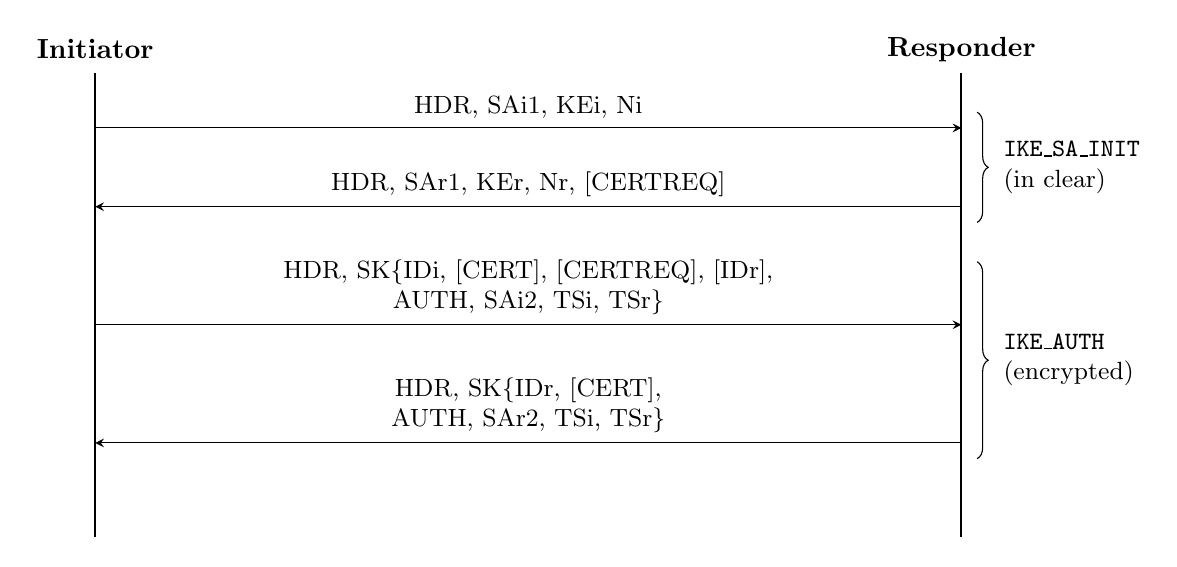
\begin{tikzpicture}[>=stealth, font=\small, x=1cm, y=1cm]
        \node[font=\bfseries] at (0,0)  {Initiator};
        \node[font=\bfseries] at (11,0) {Responder};
        \draw[thick] (0,-0.3)  -- (0,-6.2);
        \draw[thick] (11,-0.3) -- (11,-6.2);

        % IKE_SA_INIT
        \draw[->] (0,-1.0) -- node[above] {HDR, SAi1, KEi, Ni} (11,-1.0);
        \draw[<-] (0,-2.0) -- node[above] {HDR, SAr1, KEr, Nr, [CERTREQ]} (11,-2.0);
        \draw[decorate, decoration={brace, amplitude=4pt}]
            (11.2,-0.8) -- (11.2,-2.2)
            node[midway, right=6pt, align=left] {\texttt{IKE\_SA\_INIT}\\(in clear)};

        % IKE_AUTH
        \draw[->] (0,-3.5) -- node[above, align=center]
            {HDR, SK\{IDi, [CERT], [CERTREQ], [IDr],\\ AUTH, SAi2, TSi, TSr\}} (11,-3.5);
        \draw[<-] (0,-5.0) -- node[above, align=center]
            {HDR, SK\{IDr, [CERT],\\ AUTH, SAr2, TSi, TSr\}} (11,-5.0);
        \draw[decorate, decoration={brace, amplitude=4pt}]
            (11.2,-2.7) -- (11.2,-5.2)
            node[midway, right=6pt, align=left] {\texttt{IKE\_AUTH}\\(encrypted)};
    \end{tikzpicture}
    \caption{IKEv2 initial exchanges (based on RFC~7296~\cite{rfc7296}).}
    \label{fig:ikev2-flow}
\end{figure}

\paragraph{\texttt{IKE\_SA\_INIT}.}
The first exchange negotiates the cryptographic algorithms of the IKE SA,
exchanges nonces (\texttt{Ni}, \texttt{Nr}) and performs a Diffie--Hellman
exchange (\texttt{KEi}, \texttt{KEr}). The \texttt{SAi1} payload carries the
initiator's proposals, each consisting of transforms of four types:
encryption algorithm, pseudorandom function (PRF), integrity algorithm and
Diffie--Hellman group. The responder selects one proposal and returns it in
\texttt{SAr1}. Because the initiator has to guess the group for which it sends
\texttt{KEi}, a wrong guess is answered with an \texttt{INVALID\_KE\_PAYLOAD}
notification and costs an additional round trip. A responder under load may
also reply with a \texttt{COOKIE} notification, forcing the initiator to prove
reachability before the responder commits any state.

Nothing in this exchange is encrypted. Once it completes, both peers compute
the shared Diffie--Hellman secret $g^{ir}$ and derive all keys of the IKE SA:
\begin{align}
    \mathit{SKEYSEED} &= \mathrm{prf}(N_i \,|\, N_r,\; g^{ir}) \label{eq:skeyseed}\\
    \{SK_d \,|\, SK_{ai} \,|\, SK_{ar} \,|\, SK_{ei} \,|\, SK_{er} \,|\, SK_{pi} \,|\, SK_{pr}\}
        &= \mathrm{prf+}(\mathit{SKEYSEED},\; N_i \,|\, N_r \,|\, SPI_i \,|\, SPI_r)
\end{align}
$SK_{e}$ and $SK_{a}$ protect subsequent IKE messages in each direction,
$SK_{p}$ is used when computing the \texttt{AUTH} payload, and $SK_d$ is the
seed from which all Child SA keys and future IKE SA keys are derived.

\paragraph{\texttt{IKE\_AUTH}.}
The second exchange is protected with the keys derived above. The peers reveal
their identities (\texttt{IDi}, \texttt{IDr}), optionally exchange
certificates, and prove possession of their credentials in the \texttt{AUTH}
payload. This payload is a signature, or a PSK-based MAC, computed over the
sender's own \texttt{IKE\_SA\_INIT} message, the peer's nonce and
$\mathrm{prf}(SK_p, ID)$. It therefore retroactively authenticates the
unprotected first exchange and detects any tampering with it. The initiator
may instead authenticate with EAP. The same exchange also creates the first
Child SA: \texttt{SAi2}/\texttt{SAr2} negotiate the ESP or AH algorithms, and
the traffic selectors \texttt{TSi}/\texttt{TSr} define which traffic it
protects. The responder decides on the final selectors and may narrow the
initiator's proposal. The first Child SA uses the Diffie--Hellman secret of
the IKE SA, so no additional key exchange takes place. Child SA keys are
derived as
\begin{equation}
    \mathit{KEYMAT} = \mathrm{prf+}(SK_d,\; N_i \,|\, N_r). \label{eq:keymat}
\end{equation}

\paragraph{\texttt{CREATE\_CHILD\_SA}.}
Once the IKE SA is established, either peer may initiate this exchange. It serves three purposes: creating an
additional Child SA, rekeying an existing Child SA, and rekeying the IKE SA
itself. All of them may carry a fresh key exchange (\texttt{KEi},
\texttt{KEr}), and the next section discusses them in detail.

\paragraph{\texttt{INFORMATIONAL}.}
\texttt{INFORMATIONAL} exchanges carry control messages within an established
IKE SA: \texttt{Delete} payloads to close SAs, \texttt{Notify} payloads to
report errors or status, and configuration payloads. An \texttt{INFORMATIONAL}
request with an empty encrypted payload serves as a liveness check (dead peer
detection). Every \texttt{INFORMATIONAL} message must be cryptographically
protected.

\subsubsection{Rekeying and reauthentication}
\label{sec:sota-rekey}

Keys must not be used indefinitely. SAs are therefore given lifetimes, measured
in time or in the volume of protected data, and are replaced before they
expire. RFC~7296 distinguishes the following procedures.

\paragraph{Child SA rekey without key exchange.}
The initiator sends a \texttt{CREATE\_CHILD\_SA} request with a
\texttt{REKEY\_SA} notification identifying the old SA, a new SA proposal,
a fresh nonce and traffic selectors:
\[
    \text{HDR, SK\{N(REKEY\_SA), SA, Ni, TSi, TSr\}}
\]
New keys are derived according to Equation~\eqref{eq:keymat} from the fresh
nonces only. The exchange is cheap, but the new keys depend entirely on
$SK_d$. An attacker who learns $SK_d$, or the Diffie--Hellman secret of the
IKE SA, can compute them, so this variant provides no perfect forward secrecy
(PFS).

\paragraph{Child SA rekey with key exchange.}
If the request also contains a \texttt{KEi} payload (and the response
a \texttt{KEr}), a new Diffie--Hellman secret $g^{ir}_{\mathrm{new}}$ is mixed
into the derivation:
\begin{equation}
    \mathit{KEYMAT} = \mathrm{prf+}(SK_d,\; g^{ir}_{\mathrm{new}} \,|\, N_i \,|\, N_r).
\end{equation}
This gives the Child SA perfect forward secrecy with respect to the IKE SA.

\paragraph{IKE SA rekey.}
The IKE SA is rekeyed with a \texttt{CREATE\_CHILD\_SA} exchange that carries
an IKE SA proposal and a mandatory key exchange, but no traffic selectors:
\[
    \text{HDR, SK\{SA, Ni, KEi\}} \;\longrightarrow\; \text{HDR, SK\{SA, Nr, KEr\}}
\]
The new seed combines the old $SK_d$ with the new Diffie--Hellman secret:
\begin{equation}
    \mathit{SKEYSEED}_{\mathrm{new}} = \mathrm{prf}(SK_{d,\mathrm{old}},\; g^{ir}_{\mathrm{new}} \,|\, N_i \,|\, N_r).
\end{equation}
Existing Child SAs are transferred to the new IKE SA, and the old one is
deleted. The peers are \emph{not} authenticated again; their identities are
inherited from the original \texttt{IKE\_AUTH}. If both peers start a rekey
of the same SA simultaneously, the collision is resolved deterministically by
comparing nonces (Section~2.8.1 of~\cite{rfc7296}).

\paragraph{IKE SA reauthentication.}
Reauthentication re-verifies the peers' credentials, for example to detect a
revoked certificate or an expired user account. IKEv2 has no dedicated
exchange for it. Instead, a completely new IKE SA is created from scratch with
\texttt{IKE\_SA\_INIT} and \texttt{IKE\_AUTH}, all Child SAs are recreated
under it, and the old IKE SA is deleted (Section~2.8.3 of~\cite{rfc7296}).
A responder can inform the initiator of the maximum lifetime it is willing to
accept with the \texttt{AUTH\_LIFETIME} notification~\cite{rfc4478}.

\paragraph{Relevance to post-quantum migration.}
Every procedure above in which a fresh key exchange takes place is a point
where a quantum-vulnerable algorithm may be used. Protecting only the initial
\texttt{IKE\_SA\_INIT} is insufficient: if a later IKE SA rekey or a PFS Child
SA rekey uses classical Diffie--Hellman alone, an HNDL adversary can recover
the keys of every SA established from that point on. At the same time, the
\texttt{CREATE\_CHILD\_SA} exchange of RFC~7296 can carry only a single
\texttt{KE} payload, and the \texttt{IKE\_SA\_INIT} exchange is sent
unencrypted and cannot be fragmented at the IKE layer. These limitations are
what the extensions described in the next section address.

%---------------------------------------------------------------------------
\subsection{Enabling post-quantum key exchange in IKEv2}
\label{sec:sota-pqc-ike}

% NOTE: Write this section after reading the RFCs below. The bullets are
% what each subsection should answer; delete them once covered.

Introducing post-quantum algorithms into IKEv2 raises three problems. Post-quantum
public keys and ciphertexts are an order of magnitude larger than classical ones
(Table~\ref{tab:ke-sizes}). The original protocol can negotiate and carry only
one key exchange per SA. Finally, a long-term secret may be needed to protect
against HNDL even before post-quantum KEMs are deployed. The IETF IPsecME
working group has addressed each of these in a separate specification.

\subsubsection{Large messages: IKE fragmentation and \texttt{IKE\_INTERMEDIATE}}
% TODO (RFC 7383~\cite{rfc7383}):
%  - Why IP-level fragmentation is unreliable (NATs, firewalls dropping fragments).
%  - The Encrypted Fragment payload (SKF); how fragmentation is negotiated.
%  - Key limitation: only *encrypted* messages can be fragmented, so
%    IKE_SA_INIT cannot be.
% TODO (RFC 9242~\cite{rfc9242}):
%  - Where IKE_INTERMEDIATE sits (after IKE_SA_INIT, before IKE_AUTH) and why
%    it is already encrypted, and therefore fragmentable.
%  - How the content of intermediate messages is authenticated (the IntAuth
%    values added to the AUTH computation).
%  - Possibility of multiple IKE_INTERMEDIATE exchanges.

\subsubsection{Multiple key exchanges}
% TODO (RFC 9370~\cite{rfc9370}):
%  - Transform Type 4 renamed to "Key Exchange Method"; new Transform Types
%    "Additional Key Exchange 1..7".
%  - Initial SA: one additional KE per IKE_INTERMEDIATE exchange; how
%    SKEYSEED is updated after each one.
%  - CREATE_CHILD_SA: the IKE_FOLLOWUP_KE exchange (it fixes the
%    single-KE limitation described in Section~\ref{sec:sota-rekey}).
%  - Diagram: hybrid X25519 + ML-KEM initial exchange.

\subsubsection{ML-KEM in IKEv2}
% TODO (draft-ietf-ipsecme-ikev2-mlkem~\cite{ikev2mlkem}):
%  - Transform IDs for ML-KEM-512/768/1024, payload format.
%  - Mapping of KEM roles onto initiator/responder.
%  - Pure PQ vs hybrid (combined with RFC 9370), and which the draft recommends.
%  - Current status of the draft (check the datatracker before submission).

\subsubsection{Post-quantum preshared keys}
% TODO (RFC 8784~\cite{rfc8784}):
%  - The PPK and how it is mixed into SK_d, SK_pi, SK_pr.
%  - What is and is *not* protected (the initial IKE SA encryption keys).
%  - Negotiation (USE_PPK, PPK_IDENTITY), mandatory vs optional PPK.
% TODO (RFC 9867~\cite{rfc9867}):
%  - How it extends PPK mixing to IKE_INTERMEDIATE and CREATE_CHILD_SA.

\subsubsection{Post-quantum authentication}
% TODO: Short note only. Authentication with ML-DSA/SLH-DSA in IKEv2 is
% being specified separately; state it is out of scope and why
% (see Section~\ref{sec:sota-quantum}: no HNDL risk for authentication).

%---------------------------------------------------------------------------
\subsection{Implementations and related work}
\label{sec:sota-impl}
% TODO:
%  - Open-source IKEv2 daemons and their PQC support: strongSwan, Libreswan
%    (versions, which RFCs and transforms they implement). This decides
%    which VPN is chosen for the implementation part.
%  - Published measurements of PQ/hybrid IKEv2 (handshake latency, message
%    sizes, number of fragments, CPU cost), plus TLS 1.3 hybrid studies
%    for comparison.
%  - Identify what those works do *not* measure -> the gap this thesis fills.

%---------------------------------------------------------------------------
\subsection{Summary}
\label{sec:sota-summary}
% TODO: write last. 1-2 paragraphs: what is standardised, what is still a
% draft, what remains to be measured, and how this motivates the next chapter.

\clearpage
\section{Problem analysis and requirements}
\label{sec:analysis}

\subsection{Problem statement and research questions}
\label{sec:analysis-problem}
\placeholder{What exactly is measured and compared; research questions / hypotheses
(e.g.\ overhead of hybrid exchange on SA establishment and rekeying).}

\subsection{Requirements}
\label{sec:analysis-requirements}
\placeholder{Functional (interoperable hybrid exchange per RFC 9370 + ML-KEM, rekeying
support, operation on an ARM IoT-class gateway) and non-functional (reproducibility,
isolation of the test bed) requirements.}

\subsection{Selection of the IPsec implementation and hardware platforms}
\label{sec:analysis-vpn}
\placeholder{Comparison criteria and candidates (e.g.\ strongSwan, Libreswan);
justification of the choice. Hardware: x86 peer and an ARM single-board computer
acting as an IoT gateway.}

\subsection{Selection of algorithms and parameter sets}
\label{sec:analysis-algorithms}
\placeholder{Classical baseline groups, ML-KEM parameter sets, hybrid combinations
to be evaluated, and why.}

\clearpage
\section{Design and implementation}
\label{sec:impl}

\subsection{Test environment architecture}
\label{sec:impl-env}
\placeholder{Topology diagram, hosts/VMs/containers, OS and software versions,
network emulation.}

\subsection{Classical baseline configuration}
\label{sec:impl-baseline}
\placeholder{IKEv2 configuration with classical key exchange only.}

\subsection{Hybrid post-quantum configuration}
\label{sec:impl-hybrid}
\placeholder{Configuration of additional key exchanges, IKE\_INTERMEDIATE and IKE
fragmentation; build/compile steps if needed.}

\subsection{Functional verification}
\label{sec:impl-verification}
\placeholder{Evidence that the hybrid exchange really takes place: packet captures,
daemon logs, negotiated transforms.}

\clearpage
\section{Evaluation methodology}
\label{sec:method}

\subsection{Metrics}
\label{sec:method-metrics}
\placeholder{E.g.\ SA establishment time, number and size of IKE messages and
fragments, CPU and memory cost, energy per handshake on the IoT gateway,
ESP throughput (control).}

\subsection{Test scenarios}
\label{sec:method-scenarios}
\placeholder{Initial IKE SA establishment, Child SA rekey with/without key exchange,
IKE SA rekey, reauthentication; network profiles: LAN baseline and emulated
IoT links resembling LTE-M or NB-IoT (latency, bandwidth, loss, reduced MTU).}

\subsection{Measurement tools and automation}
\label{sec:method-tools}
\placeholder{Tools, scripts, number of repetitions, statistical treatment.}

\clearpage
\section{Results and analysis}
\label{sec:results}

\subsection{Initial security association establishment}
\label{sec:results-initial}
\placeholder{Results for classical vs hybrid configurations.}

\subsection{Rekeying and reauthentication}
\label{sec:results-rekey}
\placeholder{Results per rekeying procedure.}

\subsection{Impact of network conditions}
\label{sec:results-network}
\placeholder{Behaviour under latency, packet loss and reduced MTU.}

\subsection{Discussion}
\label{sec:results-discussion}
\placeholder{Interpretation, comparison with related work (Section~\ref{sec:sota-impl}),
threats to validity.}

\clearpage
\section{Summary and conclusions}
\label{sec:conclusions}

\subsection{Summary of completed work}
\label{sec:conclusions-summary}
\placeholder{What was done.}

\subsection{Critical analysis and limitations}
\label{sec:conclusions-limitations}
\placeholder{What could be done better; limits of the test bed and results.}

\subsection{Significance of the work}
\label{sec:conclusions-significance}
\placeholder{Practical value for VPN operators planning the PQC migration.}

\subsection{Future work}
\label{sec:conclusions-future}
\placeholder{E.g.\ post-quantum authentication, PPK (RFC 8784/9867), other implementations.}


%--------------
% Bibliography
%--------------
\cleardoublepage
{\sloppy\printbibliography}
\clearpage

%--------------------------------------------
% List of symbols and abbreviations
% Keep sorted alphabetically by hand.
%--------------------------------------------
\acronymlist
\acronym{AH}{Authentication Header}
\acronym{CRQC}{Cryptographically Relevant Quantum Computer}
\acronym{DH}{Diffie--Hellman}
\acronym{ECDH}{Elliptic Curve Diffie--Hellman}
\acronym{ESP}{Encapsulating Security Payload}
\acronym{HNDL}{Harvest Now, Decrypt Later}
\acronym{IETF}{Internet Engineering Task Force}
\acronym{IKE}{Internet Key Exchange}
\acronym{IPsec}{Internet Protocol Security}
\acronym{KEM}{Key Encapsulation Mechanism}
\acronym{ML-KEM}{Module-Lattice-Based Key-Encapsulation Mechanism}
\acronym{NAT}{Network Address Translation}
\acronym{NIST}{National Institute of Standards and Technology}
\acronym{PAD}{Peer Authorization Database}
\acronym{PFS}{Perfect Forward Secrecy}
\acronym{PPK}{Post-quantum Preshared Key}
\acronym{PQC}{Post-Quantum Cryptography}
\acronym{PSK}{Pre-Shared Key}
\acronym{SA}{Security Association}
\acronym{SAD}{Security Association Database}
\acronym{SPD}{Security Policy Database}
\acronym{SPI}{Security Parameter Index}
\acronym{VPN}{Virtual Private Network}
\vspace{0.8cm}

%---------------------------------
% Lists of figures, tables, appendices
%---------------------------------
\pagestyle{plain}

\listoffigurestoc
\vspace{1cm}
\listoftablestoc
\vspace{1cm}
\listofappendicestoc

%------------
% Appendices
%------------

% Figures and tables in appendices are not listed
\captionsetup[figure]{list=no}
\captionsetup[table]{list=no}

\clearpage
\appendix{Test environment configuration}
\placeholder{Full IKEv2 daemon configuration files for the classical and hybrid setups.}

\clearpage
\appendix{Measurement scripts}
\placeholder{Scripts used to run the experiments and process the results.}

\end{document}
